% ----------------------------------------------------------
% PARTE
% ----------------------------------------------------------
\part{Resultados}
% ----------------------------------------------------------

\chapter{Case: Loan Club}

\section{Loan Club}

A Loan Club é um marketplace de créditos online. Trata-se de uma plataforma que reune pessoas que gostariam de realizar um empréstimo e outras que possuem um capital a investir. Em geral, são empréstimos pessoais, de negócios ou para procedimentos médicos. A proposta é oferecer um serviço de fácil acesso via dispositivos mobiles a taxa baixas, além de garantir um retorno que se ajuste a expectativa do investidor. Dessa forma, operam de forma menos burocrática do que um banco mas assumindo os riscos de uma instituição financeira.

\section{Kaggle}

Kaggle é uma plataforma criada em 2010 que reune ferramentas e estudos sobre modelagem preditiva. Também viabiliza competições de temas relacionados a análise preditiva. Com o intuito de compartilhar conhecimento, qualquer interessado pode acessar dados de empresas para aplicar estudos ou gerar novos modelos. Além disso, o Kaggle também tem sido usado como uma forma de recrutar cientistas de dados. A base da Loan Club foi disponibilizado no Kaggle e usado como objeto de estudo deste trabalho.

\section{Tecnologias}

\subsection{Scikit Learn}

O Scikit Learn é um framework desenvolvido em Python voltado para Data Science. Com mais de 30 contribuidores ativos, possui implementação de diversos algoritmos e de ferramentas que auxiliam desde a análise dos dados até na execução de tarefas como clusterização e classificação até a execução dos algoritmos de Machine Learning, além de disponiblizar integrações com programas visuais que facilitam muito a compreensão. 


\subsection{Apache Spark}

O Apache Spark é uma biblioteca com diversas ferramentas, entre elas que viabiliza a escalabilidade da execução de algoritmos de Machine Learning. Os algoritmos estudados (em especial o K Médias) são robustos e possuem uma grande carga de cáculos. Para bases grandes, o Scikit Learn não é capaz de executar em tempo satisfatório. O Apache Spark, por outro lado, oferece uma solução que possibilita uma maior rapidez na execução. Também é possível configurá-lo para que os algoritimos sejam executados em tempo real com alimentação contínua de dados. Contudo tal abordagem não será contemplada por não se tratar do foco do estudo.

\section{Preparação da base}

Como uma base de uma empresa, o Loan Club apresenta diversos problemas como:

\subsection{Missing values}
Inerente a uma base comum de qualquer empresa, missing values ocorre quando uma informação não consta na base. Esse fato pode influenciar a conclusão de uma análise porque a ausência de dados pode distorcê-la. Para diminuir o impacto desse tipo de problema, é necessário verificar a natureza da informação. Elas são oriundas desde problemas do armazenamento da informação, provenientes desde erros humanos, falta de informação ou em decorrência de algum problema ou inconsistência no sistema de informação.

Para os algoritmos, é necessário que algum valor seja colocado para a realização dos cálculos. Há diversas abordagens, como substituição por um valor padrão que faça sentido para cada informação. Em alguns casos, são usados valores como 0, média ou moda dos campos respectivos das observações. Contudo, é evidente que cada uma dessas técnicas enviesa e modifica o resultado. Neste estudo, desprezamos as informações que possuiam altas ocorrências de missing values e para as que possuiam menos de 1\% de missing values, foi preenchido com 0. 

\subsection{Conversão de tipo de dados}
Alguns dados como int\_rate ou o term estavam armazenados como tipo texto, sendo inviável a execução do algoritmo do K Médias. Para isso, foram removidos termos de texto e converteu-se os valores em número.


\subsection{Remoção das variáveis categóricas}
O algoritmo de K Médias, a princípio, não é executado com uma base que contenha variáveis categóricas. É possível adaptar a base executando uma transformação, tornando-as variáveis dummies. Contudo, não iremos considerar as variáveis categóricas por haver uma carga considerável e inviável de trabalho no escopo deste estudo. A Random Forest consegue lidar com variáveis categóricas mas também necessita de algumas transformações mas que não foram feitas neste trabalho.


\section{Avaliação dos algoritmos}

\subsection{Segmentação}

\subsubsection{Análise Descritiva}
A análise descritiva possibilita a descrição e sumarização dos dados de um conjunto. Há 2 tipos de medidas: a de tendência central e a de variabilidade ou dispersão. Entre as medidas de tendência central estão média, mediana e moda. Já para as medidas de variabilidade, existem o desvio padrão, variância, o valor máximo e mínimo e quantis.
Para a análise descritiva, pode-se utilizar gráficos como histogramas e boxplots que ajudam visualizar com clareza e caracterizar dos dados.


\subsection{Classificação}

\subsubsection{Cross Validation}

A Cross Validation é uma técnica que permite verificar a acurácia de um modelo preditivo. A idéia é particionar a base para se criar um modelo de treinamento e executar um teste. Essa partição é mutualmente exclusiva, ou seja, os dados que são usados para o treinamento não são reutilizados no teste. Neste caso, a Cross Validation será executada nos algoritmos de classificação.


\subsubsection{Métricas}
O cálculo de métricas para os algoritmos são importantes para avaliar o desempenho da segmentação e da classificação. Cada métrica pode ser mais conveniente para cada tipo de problema ou natureza dos dados. Neste trabalho iremos abordar algumas métricas simples.

\subsubsection{Precision}

É calculado a partir da proporção dos verdadeiros positivos sobre a quantidade de todos elementos que foram classificados na mesma classe (soma dos verdadeiros positivos e falsos positivos)

\begin{equation}
  \label{eq:precision}
  \begin{aligned}
Precision &= \frac{VP}{VP + FP} 
  \end{aligned}  
\end{equation}

\subsubsection{Recall}

É a proporção de elementos foram classificados corretamente em uma classe 
sobre a quantidade de todos elementos que realmente pertencem a esta classe mesmo que estejam em outras (soma dos verdadeiros positivos e falsos negativos). 

\begin{equation}
  \label{eq:precision}
  \begin{aligned}
Recall &= \frac{VP}{VP + FN} 
  \end{aligned}  
\end{equation}

\subsubsection{Falso Positivo}
\lipsum[27]

\subsubsection{F-measure}
O F-measure é a média harmônica entre precisão e recall. Trata-se de uma medida que consegue avaliar melhor conjunto de dados que possuem uma distribuição das classes desproporcionais. 

\begin{equation}
  \label{eq:precision}
  \begin{aligned}
F-measure &= (1 + \beta^{2})\frac{precision*recall}{\beta^{2}*precision + recall} 
  \end{aligned}  
\end{equation}

\subsubsection{Confusion Matrix}
Trata-se de uma matriz quadrada na qual 
as colunas representam as classes as quais o elementos realmente pertencem enquanto as linhas representa a saída do classificador. Cada célula fornece a quantidade de elementos classificados.

\section{Algoritmos}

\subsection{K Médias}

O objetivo de uma clusterização é para dado um conjunto de dados e agrupar os elementos em grupos baseados na similaridade entre eles. Com a base de dados da Loan Club, já contamos com uma divisão feita por ela mesma. Dessa forma, uma hipótese a ser testada é constatar alguma relação nos grupos gerados pelo K Médias com alguma característica. Neste trabalho, iremos usar as notas atribuídas por ela mesma, armazenada no campo \emph{grade}.

Para a execução do K Médias, executou-se uma normalização dos dados. Ela é recomendada pois como os dados possuem diversas informações, é possível que haja grandes disparidades de intervalos. Assim quando se normaliza todos os dados, a idéia é uniformizar esses intervalos para que não haja muita interferência nos cálculos do algoritmo. 

\subsubsection{Scikit Learn}

Pelo Scikit Learn, é possível criar gráficos de boxplot para visualizar em quais campos houve uma separação mais clara do banco. Inicialmente foi feito criado uma amostra de 8000 registros na qual foi executado o K Médias. Esses gráficos estão disponível em Anexos na seção Análise dos clusters vs grades. Junto desses gráficos, há um comparativo com boxplots gerados a partir dos grades estabelecidos pela Loan Club. Dessa forma, pode-se ver que existe uma relação entre os clusters e os grades.

Campos como o funded\_amnt, installment, loan\_amnt, total\_pymnt deixam muito claro a segregação dos clusters, enquanto que os outros não foram capazes de mostrar a diferença entre os grupos.
Não foi possível criar esses gráficos para a base toda pois seria necessário uma integração entre as ferramentas do Scikit Learn e do Apache Spark uma vez que não foi possível clusterizar toda a base via Scikit Learn. Contudo, devemos ressaltar que dentro de um contexto de Big Data nem sempre será possível utilizar as ferramentas de visualização por conta da quantidade de dados.


\begin{figure*}[!ht]
    \centering
        \caption{funded\textunderscore amnt }
        \begin{subfigure}[t]{0.45\textwidth}
            \centering
            \caption{Cluster }

            \centerline{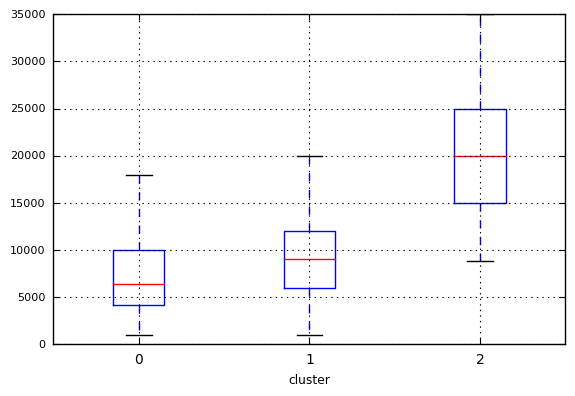
\includegraphics[width=1\textwidth]{img/funded_amnt_by_cluster}}
        \end{subfigure}%
        ~ 
        \begin{subfigure}[t]{0.45\textwidth}
            \centering
            \caption{Grade }
   
            \centerline{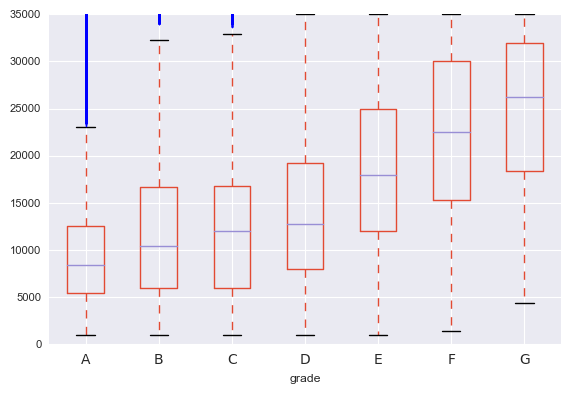
\includegraphics[width=1\textwidth]{img/funded_amnt_by_grade}}

        \end{subfigure}
\end{figure*}

\begin{figure*}[!ht]
    \centering        
                \caption{installment}
        \begin{subfigure}[t]{0.45\textwidth}
            \centering

            \centerline{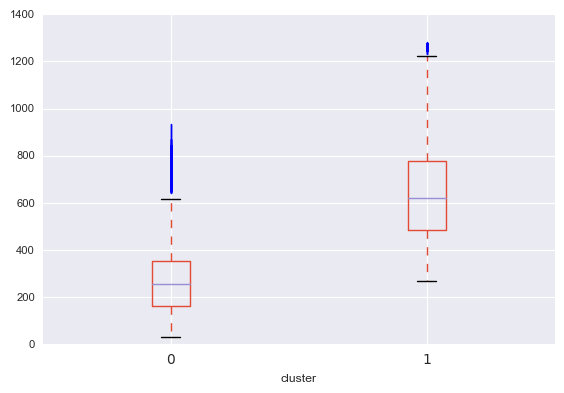
\includegraphics[width=1.05\textwidth]{img/installment_by_cluster}}
        \end{subfigure}%
        ~ 
        \begin{subfigure}[t]{0.45\textwidth}
            \centering
   
            \centerline{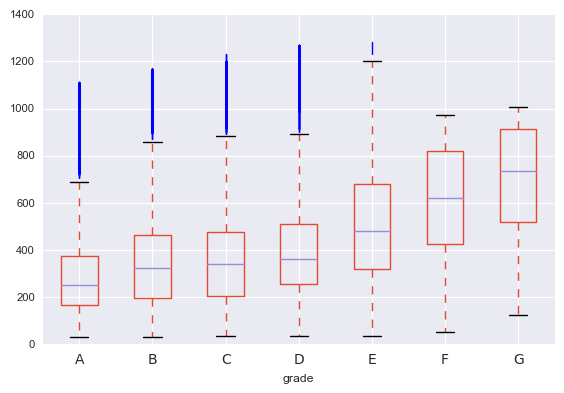
\includegraphics[width=1.05\textwidth]{img/installment_by_grade}}

        \end{subfigure}

\end{figure*}


\begin{figure*}[!ht]
    \centering
        \caption{loan\textunderscore amnt }
        \begin{subfigure}[t]{0.45\textwidth}
            \centering
            \caption{Cluster }

            \centerline{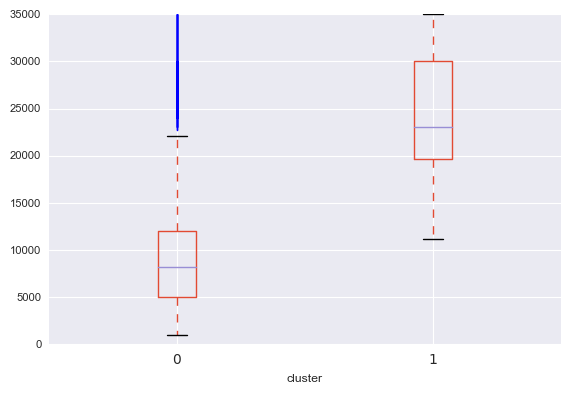
\includegraphics[width=1\textwidth]{img/loan_amnt_by_cluster}}
        \end{subfigure}%
        ~ 
        \begin{subfigure}[t]{0.45\textwidth}
            \centering
            \caption{Grade }
   
            \centerline{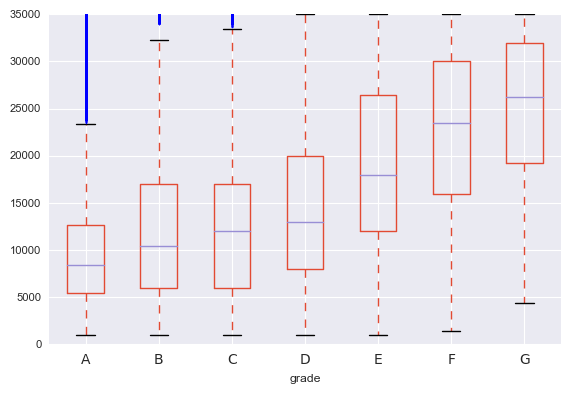
\includegraphics[width=1\textwidth]{img/loan_amnt_by_grade}}

        \end{subfigure}

\end{figure*}


\begin{figure*}[!ht]
    \centering
                \caption{total\textunderscore pymnt}
        \begin{subfigure}[t]{0.45\textwidth}
            \centering

            \centerline{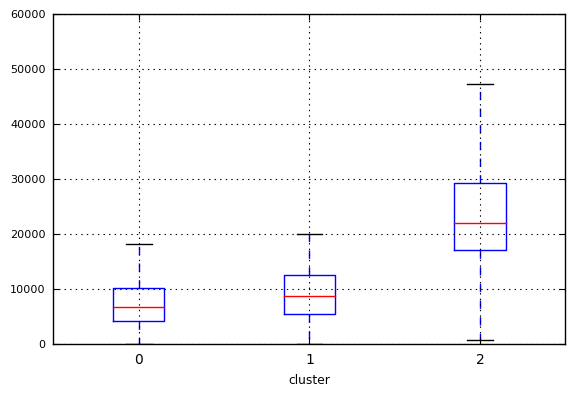
\includegraphics[width=1.05\textwidth]{img/total_pymnt_by_cluster}}
        \end{subfigure}%
        ~ 
        \begin{subfigure}[t]{0.45\textwidth}
            \centering
   
            \centerline{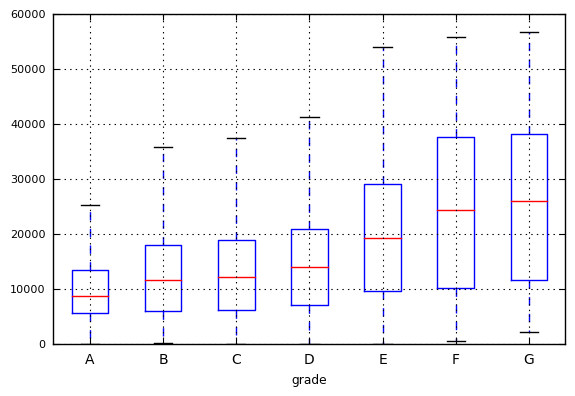
\includegraphics[width=1.05\textwidth]{img/total_pymnt_by_grade}}

        \end{subfigure}

\end{figure*}

\subsubsection{Apache Spark}

Pelo Apache Spark, é possível calcular algumas váriaveis como a média, o desvio padrão, mínimo e máximo sobre a base completa. Na tabela abaixo, comparamos os 4 componentes de cada cluster.

\pagebreak

\begin{table}
\tiny
\centering
        \caption{Média, Desvio Padrão, Mínimo, Máximo dos Clusters}
        \label{multiprogram}
        \begin{tabular}{c | c c c | c c c | c c c | c c c } \toprule
             Variável & \multicolumn{3}{|c|}{Média} & \multicolumn{3}{|c|}{Desvio Padrão} & \multicolumn{3}{|c|}{Mínimo} & \multicolumn{3}{|c}{Máximo}\\
             & 1 & 2 & 3 & 1 & 2 & 3 & 1 & 2 & 3 & 1 & 2 & 3\\
             \hline
            \multicolumn{1}{c|}{1} & 1.103  & 1.038  & -0.598 & 0.730 & 0.741 & 0.513 & -0.562 & -1.639 & -1.689 & 2.403   & 2.403   & 2.403  \\
            \multicolumn{1}{c|}{2} & 1.099  & 1.039  & -0.598 & 0.733 & 0.742 & 0.514 & -1.729 & -1.742 & -1.742 & 2.404   & 2.404   & 1.812  \\
            \multicolumn{1}{c|}{3} & 1.106  & 1.037  & -0.598 & 0.729 & 0.741 & 0.514 & -0.563 & -1.639 & -1.690 & 2.399   & 2.399   & 2.399  \\
            \multicolumn{1}{c|}{4} & 0.331  & 0.659  & -0.311 & 1.085 & 1.067 & 0.794 & -0.654 & -0.654 & -0.654 & 1.527   & 1.527   & 1.527  \\
            \multicolumn{1}{c|}{5} & 0.469  & 0.259  & -0.185 & 1.063 & 1.074 & 0.903 & -1.809 & -1.809 & -1.809 & 3.592   & 3.592   & 3.592  \\
            \multicolumn{1}{c|}{6} & 1.164  & 0.892  & -0.554 & 0.885 & 0.852 & 0.532 & -0.748 & -1.665 & -1.724 & 3.985   & 4.131   & 2.880  \\
            \multicolumn{1}{c|}{7} & 0.338  & 0.372  & -0.204 & 0.956 & 1.546 & 0.609 & -0.788 & -1.159 & -1.141 & 76.122  & 145.675 & 91.578 \\
            \multicolumn{1}{c|}{8} & -0.071 & 0.115  & -0.030 & 0.430 & 1.833 & 0.497 & -1.056 & -1.056 & -1.056 & 1.268   & 580.557 & 62.492 \\
            \multicolumn{1}{c|}{9} & -0.036 & 0.034  & -0.006 & 0.905 & 1.024 & 1.006 & -0.364 & -0.364 & -0.364 & 27.471  & 29.791  & 44.869 \\
            \multicolumn{1}{c|}{10} & 0.121  & 0.053  & -0.042 & 1.081 & 1.057 & 0.958 & -0.696 & -0.696 & -0.696 & 10.331  & 32.385  & 26.370 \\
            \multicolumn{1}{c|}{11} & 0.003  & 0.461  & -0.175 & 0.882 & 1.139 & 0.903 & -2.172 & -2.172 & -2.172 & 7.983   & 14.754  & 9.488  \\
            \multicolumn{1}{c|}{12} & -0.159 & 0.060  & 0.006  & 0.698 & 1.341 & 0.886 & -0.335 & -0.335 & -0.335 & 35.739  & 147.398 & 16.842 \\
            \multicolumn{1}{c|}{13} & 0.295  & 0.429  & -0.217 & 1.133 & 1.528 & 0.553 & -0.754 & -0.754 & -0.754 & 52.312  & 128.779 & 21.998 \\
            \multicolumn{1}{c|}{14} & 0.088  & 0.533  & -0.219 & 0.896 & 1.083 & 0.901 & -1.965 & -1.880 & -2.049 & 7.663   & 12.139  & 7.071  \\
            \multicolumn{1}{c|}{15} & -0.483 & 1.243  & -0.383 & 0.842 & 0.928 & 0.573 & -0.989 & -0.989 & -0.989 & 2.713   & 4.823   & 1.763  \\
            \multicolumn{1}{c|}{16} & -0.483 & 1.243  & -0.383 & 0.842 & 0.928 & 0.573 & -0.989 & -0.989 & -0.989 & 2.714   & 4.825   & 1.764  \\
            \multicolumn{1}{c|}{17} & 2.129  & -0.218 & -0.310 & 0.938 & 0.573 & 0.569 & 0.121  & -0.960 & -0.960 & 6.379   & 4.054   & 2.658  \\
            \multicolumn{1}{c|}{18} & 2.131  & -0.215 & -0.311 & 0.941 & 0.573 & 0.567 & -0.943 & -0.958 & -0.958 & 6.404   & 3.855   & 1.837  \\
            \multicolumn{1}{c|}{19} & 2.052  & -0.332 & -0.253 & 1.114 & 0.494 & 0.597 & -0.869 & -0.869 & -0.869 & 4.413   & 4.413   & 2.904  \\
            \multicolumn{1}{c|}{20} & 1.507  & 0.216  & -0.360 & 1.657 & 0.894 & 0.430 & -0.837 & -0.837 & -0.837 & 10.713  & 6.837   & 2.927  \\
            \multicolumn{1}{c|}{21} & 0.112  & -0.005 & -0.018 & 1.757 & 1.076 & 0.742 & -0.097 & -0.097 & -0.097 & 87.747  & 72.073  & 59.306 \\
            \multicolumn{1}{c|}{22} & 0.015  & 0.071  & -0.029 & 1.474 & 1.360 & 0.676 & -0.112 & -0.112 & -0.112 & 81.709  & 67.624  & 53.445 \\
            \multicolumn{1}{c|}{23} & 0.027  & 0.046  & -0.022 & 1.488 & 1.286 & 0.724 & -0.077 & -0.077 & -0.077 & 110.893 & 82.221  & 91.441 \\
            \multicolumn{1}{c|}{24} & 1.469  & -0.281 & -0.164 & 2.008 & 0.326 & 0.567 & -0.451 & -0.451 & -0.451 & 7.155   & 7.006   & 5.194 \\\bottomrule
        \end{tabular}
        \fonte{Dados gerados pelo script}
    \end{table}

Assim como nos boxplots do Anexo, é possível notar pela tabela que algumas variáveis não possuem valores que viabilize a criação de clusters por si só.
Podemos observar uma nítida diferença entre os clusters 1 e 3, sendo que o cluster 2 possui algumas variáveis mais próximas do cluster 1 e para outras, mais próxima do cluster 3.


\subsection{Regressão Logística}


\subsubsection{Spark}

A execução da Regressão Logística foi dividida em 2 fases: treinamento do modelo e teste. A base completa foi dividida em 80\% para treino e 20 \% para testes. Para verificar a clssificação, foi considerado a clusterização realizada previamente pelo K Médias. 

%\begin{tabular}{ r r r r }

 %        & 1 & 2 & 3 \\
 %   1    & 29585 & 334   & 1307  \\
 %   2    & 715   & 58836 & 3957  \\
 %   3    & 1342  & 5006  & 164590
%\end{tabular}

%Também conhecida como matriz de erros, a confusion matrix é uma representação visual dos erros ocorridos durante o processamento do algoritmo. As linhas representam a classe que o dado pertence e a coluna representa a classificação gerada durante o processo. Quando um registro não está dentro da diagonal principal, significa que o algoritmo fez uma classificação diferente do que foi esperado.

%\begin{figure}[!ht]
%\caption{Confusion Matrix}
%\centerline{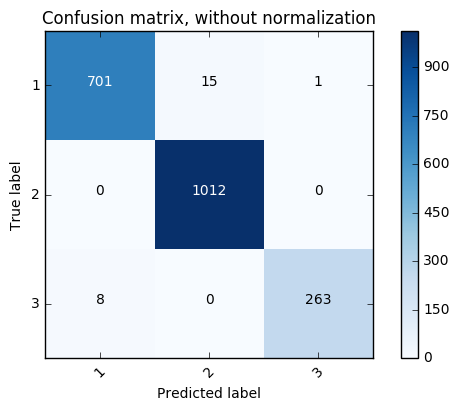
\includegraphics[width=.6\textwidth]{img/confusionMatrix}}
%\fonte{Gerado a partir do script}
%\end{figure}

\begin{figure}[!ht]
    \centering
        \caption{Resultados da clusterização da Regressão Logística}
    \begin{subfigure}[t]{0.45\textwidth}
        \centering
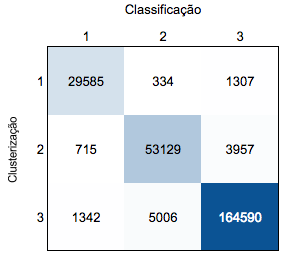
\includegraphics[width=1\linewidth]{CM-RL-abs.png}

        \caption{Classificação em valores absolutos}
    \end{subfigure}%
    ~ 
    \begin{subfigure}[t]{0.45\textwidth}
        \centering
        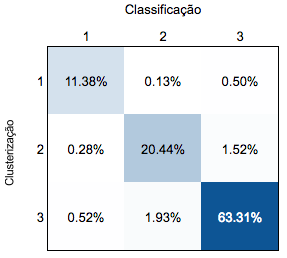
\includegraphics[width=1\linewidth]{CM-RL-per.png}
        \caption{Classificação em percentual}
    \end{subfigure}

\fonte{Gerado a partir do script}
\end{figure}

Podemos notar que houve uma classificação com baixos índices de erros, isto é, com menos de 5\% de predições em classes não esperadas. A classificação dos registros seguiu uma proporção de 11,38\% para a classe 1, 20,44\% para a classe 2 e 63,31\% para a classe 3.

\begin{table}[!ht]
  \caption{Métricas para a Regressão Logística}
  \centering
  \begin{tabular}{ c c c c c } \toprule
  Classe & Precisão & Recall  & Falso Positivo & F-measure  \\\midrule
    1    & 0,93499  & 0,94744 & 0,00877        & 0,94117    \\
    2    & 0,91679  & 0,92643 & 0,02641        & 0,95234    \\
    3    & 0,96900  & 0,96286 & 0,05556        & 0,95241 \\\bottomrule
\end{tabular}
\fonte{Tabela gerada pelo script}
\end{table}

\subsection{Random Forest}


\subsubsection{Scikit Learn}

Com uma árvore de decisão tem-se uma representação visual, de fácil interpretação de como é feito a classificação. Foi possível construir uma árvore para ilustrar a árvore do Loan Club. Neste caso, foi feito uma redução de dimensionalidade para 2 features, considerando-se 3 clusters.



\begin{figure}[!ht]
\caption{Estrutura da arvore de decisao com dimensionalidade reduzida para 2 features}
\centerline{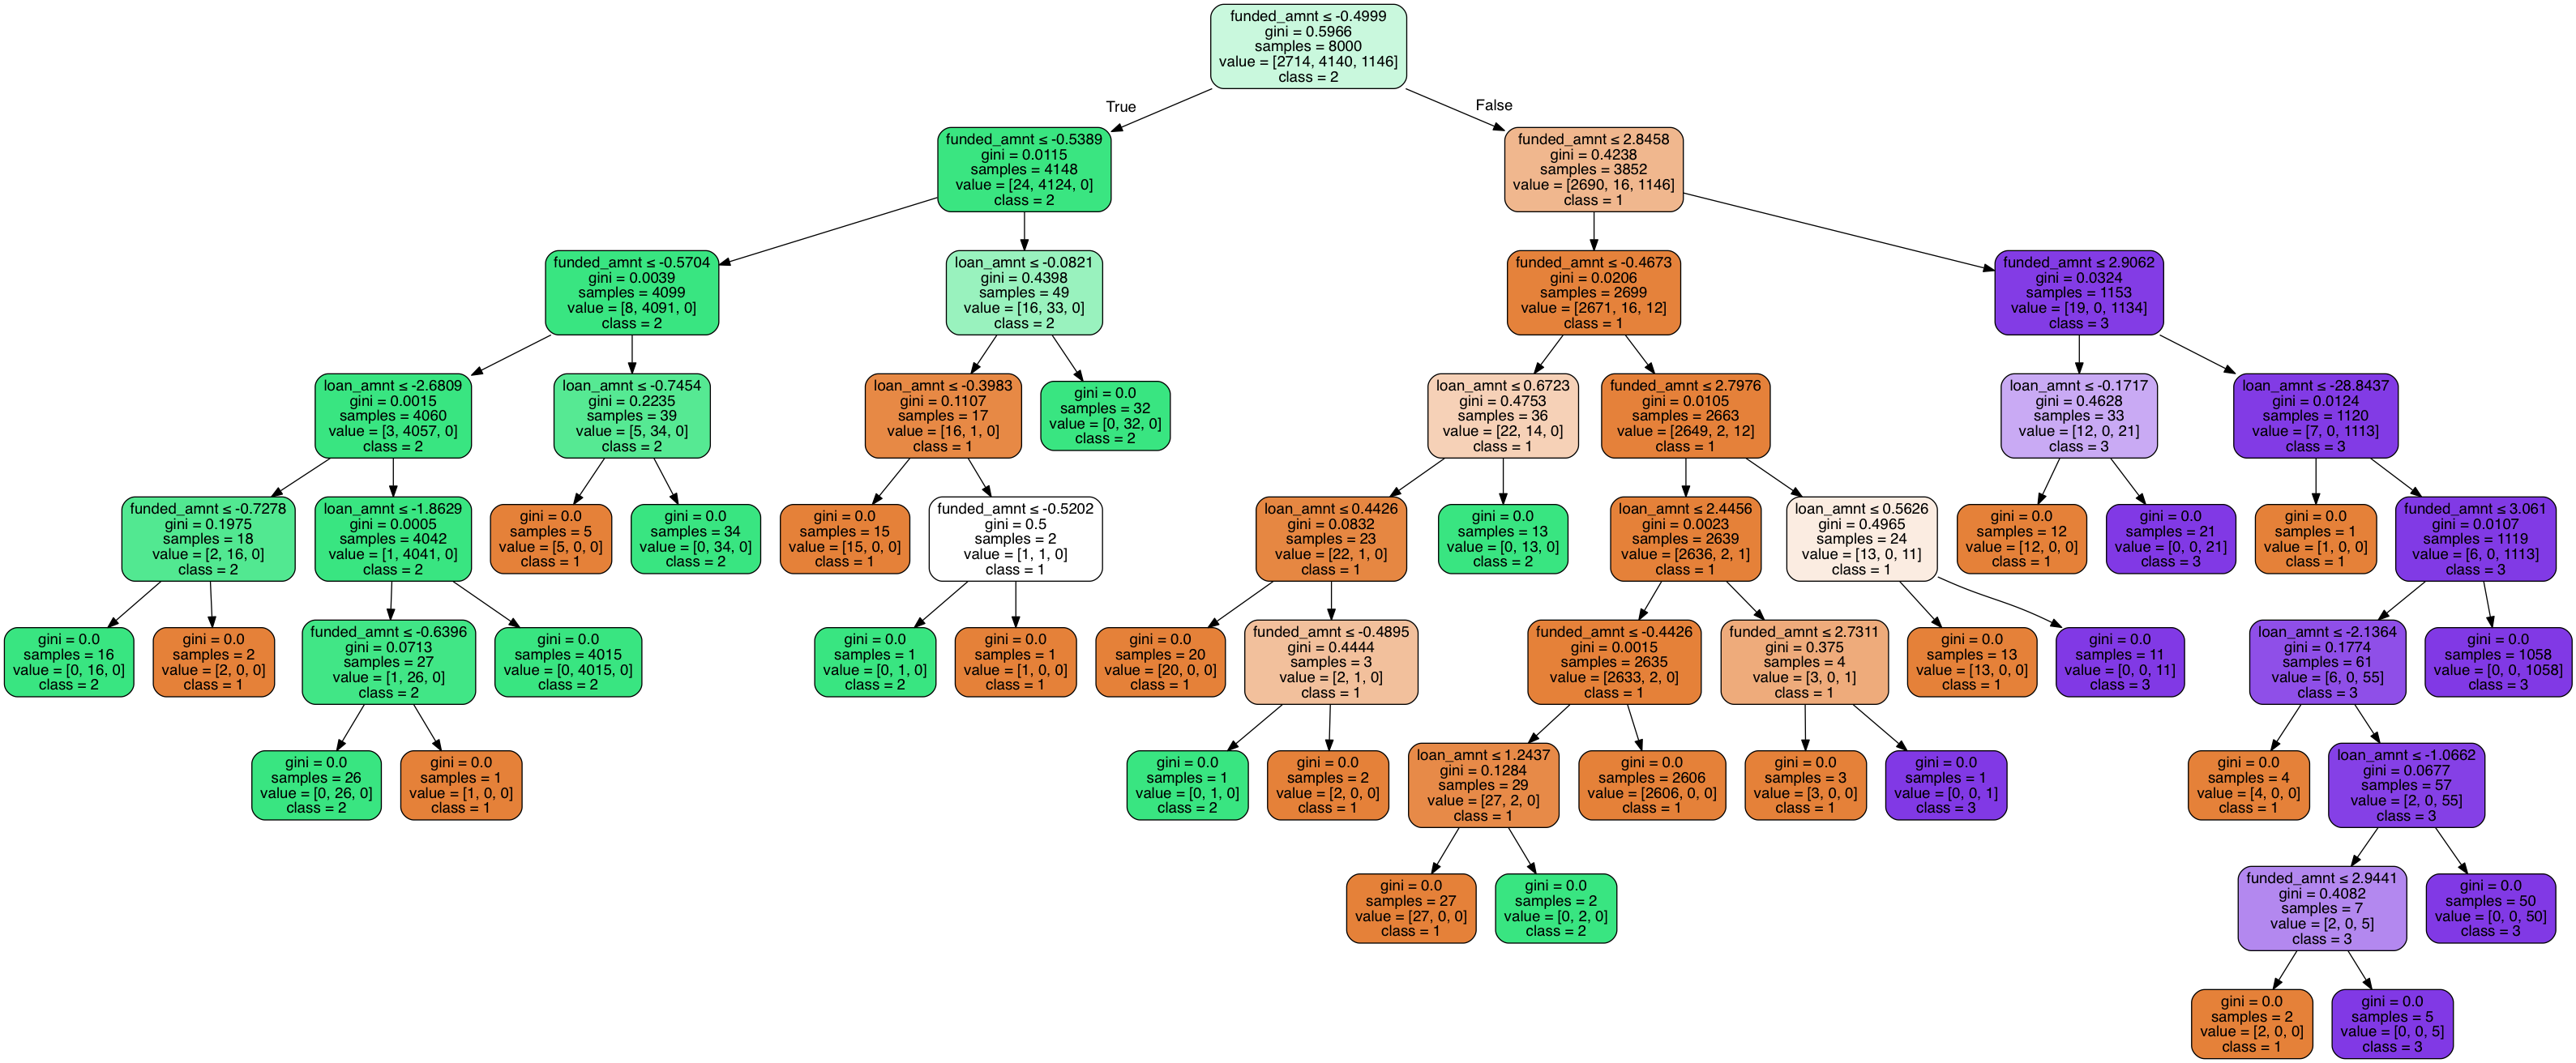
\includegraphics[width=.7\textwidth]{img/loan}}
\fonte{Gerado a partir do script}
\end{figure}

A árvore para mais de 20 features fica muito maior por conta da quantidade de informações.


Ao gerar uma árvore de classificação, o algoritmo também disponibiliza a relevância das features.

\begin{figure}[!ht]
\caption{Features mais relevantes}
\centerline{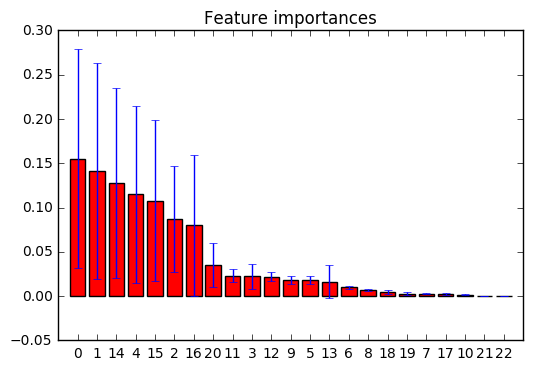
\includegraphics[width=.7\textwidth]{img/tree-most-important-features}}
\fonte{Gerado a partir do script}
\end{figure}

Desta base, é possível notar que 8 destas features possuem maior relevância frente as demais. Isso pode levar a uma redução de dimensionalidade, isto é, as features de menor relevância passam a ser descartadas no treinamento do modelo, o que pode gerar economia de processamento de dados. Por outro lado, isso é válido partindo-se do pressuposto de que a natureza das informações se manterão, o que pode não ser verdade.

%
%\lstinputlisting[language=Python, firstline=37, lastline=45]{
%load_data.py
%}

\subsubsection{Apache Spark}

%\begin{figure}[!ht]
%\caption{Confusion Matrix}
%\centerline{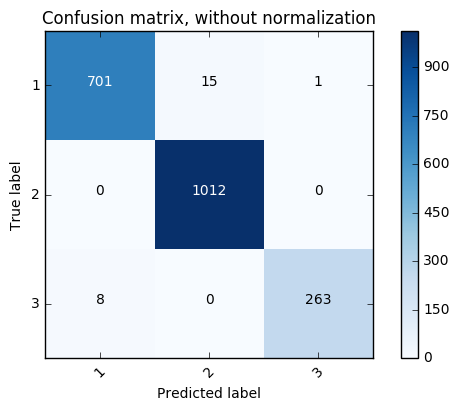
\includegraphics[width=.6\textwidth]{img/confusionMatrix}}
%\fonte{Gerado a partir do script}
%\end{figure}

Assim como na Regressão Logística, a classificação com Random Forest também foi dividida em 2 fases: treinamento do modelo (80 \%) e teste (20 \%). Para verificar a classificação, foi considerado a clusterização realizada previamente pelo K Médias. 



\begin{figure}[!ht]
    \centering
        \caption{Resultados da clusterização da Random Forest}
    \begin{subfigure}[t]{0.45\textwidth}
        \centering
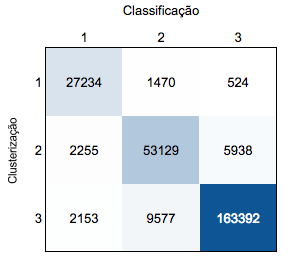
\includegraphics[width=1\linewidth]{CM-RF-abs.png}

        \caption{Classificação em valores absolutos}
    \end{subfigure}%
    ~ 
    \begin{subfigure}[t]{0.45\textwidth}
        \centering
        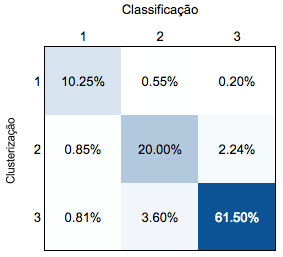
\includegraphics[width=1\linewidth]{CM-RF-per.png}
        \caption{Classificação em percentual}
    \end{subfigure}

\fonte{Gerado a partir do script}
\end{figure}

Ao compararmos com a classificação realizada pela Regressão Logística, percebe-se que também houve baixos índices de erros, isto é, com menos de 7\% de predições em classes não esperadas. Manteve-se uma proporção das classes muito próxima ao da Regressão Logística: 10,25\% para a classe 1, 20,00\% para a classe 2 e 61,50\% para a classe 3.



\begin{table}[!ht]
  \caption{Métricas para a Random Forest}
  \centering
  \begin{tabular}{ c c c c c } \toprule
  Classe & Precisão & Recall  & Falso Positivo & F-measure  \\\midrule
        1    & 0,86069  & 0,93177 & 0,01864        & 0,89482    \\
    2    & 0,82786  & 0,86639 & 0,05405        & 0,84669    \\
    3    & 0,96195  & 0,93301 & 0,07136        & 0,94726 \\\bottomrule
\end{tabular}
\end{table}


% ---
% primeiro capitulo de Resultados
% ---
%\chapter{Lectus lobortis condimentum}
% ---

% ---
%\section{Vestibulum ante ipsum primis in faucibus orci luctus et ultrices
%posuere cubilia Curae}
% ---

%\lipsum[21-22]

% ---
% segundo capitulo de Resultados
% ---
%\chapter{Nam sed tellus sit amet lectus urna ullamcorper tristique interdum
%elementum}
% ---

% ---
%\section{Pellentesque sit amet pede ac sem eleifend consectetuer}
% ---

%\lipsum[24]

% ----------------------------------------------------------
% Finaliza a parte no bookmark do PDF
% para que se inicie o bookmark na raiz
% e adiciona espaço de parte no Sumário
% ----------------------------------------------------------
%\phantompart